% Generated by Sphinx.
\def\sphinxdocclass{report}
\documentclass[letterpaper,10pt,openany,oneside]{sphinxmanual}
\usepackage[utf8]{inputenc}
\DeclareUnicodeCharacter{00A0}{\nobreakspace}
\usepackage[T1]{fontenc}
\usepackage[english]{babel}
\usepackage{times}
\usepackage[Bjarne]{fncychap}
\usepackage{longtable}
\usepackage{sphinx}
\usepackage{multirow}


\title{CDS\_java Documentation}
\date{July 13, 2012}
\release{}
\author{CSInParallel Project}
\newcommand{\sphinxlogo}{}
\renewcommand{\releasename}{}
\makeindex

\makeatletter
\def\PYG@reset{\let\PYG@it=\relax \let\PYG@bf=\relax%
    \let\PYG@ul=\relax \let\PYG@tc=\relax%
    \let\PYG@bc=\relax \let\PYG@ff=\relax}
\def\PYG@tok#1{\csname PYG@tok@#1\endcsname}
\def\PYG@toks#1+{\ifx\relax#1\empty\else%
    \PYG@tok{#1}\expandafter\PYG@toks\fi}
\def\PYG@do#1{\PYG@bc{\PYG@tc{\PYG@ul{%
    \PYG@it{\PYG@bf{\PYG@ff{#1}}}}}}}
\def\PYG#1#2{\PYG@reset\PYG@toks#1+\relax+\PYG@do{#2}}

\def\PYG@tok@gd{\def\PYG@tc##1{\textcolor[rgb]{0.63,0.00,0.00}{##1}}}
\def\PYG@tok@gu{\let\PYG@bf=\textbf\def\PYG@tc##1{\textcolor[rgb]{0.50,0.00,0.50}{##1}}}
\def\PYG@tok@gt{\def\PYG@tc##1{\textcolor[rgb]{0.00,0.25,0.82}{##1}}}
\def\PYG@tok@gs{\let\PYG@bf=\textbf}
\def\PYG@tok@gr{\def\PYG@tc##1{\textcolor[rgb]{1.00,0.00,0.00}{##1}}}
\def\PYG@tok@cm{\let\PYG@it=\textit\def\PYG@tc##1{\textcolor[rgb]{0.25,0.50,0.56}{##1}}}
\def\PYG@tok@vg{\def\PYG@tc##1{\textcolor[rgb]{0.73,0.38,0.84}{##1}}}
\def\PYG@tok@m{\def\PYG@tc##1{\textcolor[rgb]{0.13,0.50,0.31}{##1}}}
\def\PYG@tok@mh{\def\PYG@tc##1{\textcolor[rgb]{0.13,0.50,0.31}{##1}}}
\def\PYG@tok@cs{\def\PYG@tc##1{\textcolor[rgb]{0.25,0.50,0.56}{##1}}\def\PYG@bc##1{\colorbox[rgb]{1.00,0.94,0.94}{##1}}}
\def\PYG@tok@ge{\let\PYG@it=\textit}
\def\PYG@tok@vc{\def\PYG@tc##1{\textcolor[rgb]{0.73,0.38,0.84}{##1}}}
\def\PYG@tok@il{\def\PYG@tc##1{\textcolor[rgb]{0.13,0.50,0.31}{##1}}}
\def\PYG@tok@go{\def\PYG@tc##1{\textcolor[rgb]{0.19,0.19,0.19}{##1}}}
\def\PYG@tok@cp{\def\PYG@tc##1{\textcolor[rgb]{0.00,0.44,0.13}{##1}}}
\def\PYG@tok@gi{\def\PYG@tc##1{\textcolor[rgb]{0.00,0.63,0.00}{##1}}}
\def\PYG@tok@gh{\let\PYG@bf=\textbf\def\PYG@tc##1{\textcolor[rgb]{0.00,0.00,0.50}{##1}}}
\def\PYG@tok@ni{\let\PYG@bf=\textbf\def\PYG@tc##1{\textcolor[rgb]{0.84,0.33,0.22}{##1}}}
\def\PYG@tok@nl{\let\PYG@bf=\textbf\def\PYG@tc##1{\textcolor[rgb]{0.00,0.13,0.44}{##1}}}
\def\PYG@tok@nn{\let\PYG@bf=\textbf\def\PYG@tc##1{\textcolor[rgb]{0.05,0.52,0.71}{##1}}}
\def\PYG@tok@no{\def\PYG@tc##1{\textcolor[rgb]{0.38,0.68,0.84}{##1}}}
\def\PYG@tok@na{\def\PYG@tc##1{\textcolor[rgb]{0.25,0.44,0.63}{##1}}}
\def\PYG@tok@nb{\def\PYG@tc##1{\textcolor[rgb]{0.00,0.44,0.13}{##1}}}
\def\PYG@tok@nc{\let\PYG@bf=\textbf\def\PYG@tc##1{\textcolor[rgb]{0.05,0.52,0.71}{##1}}}
\def\PYG@tok@nd{\let\PYG@bf=\textbf\def\PYG@tc##1{\textcolor[rgb]{0.33,0.33,0.33}{##1}}}
\def\PYG@tok@ne{\def\PYG@tc##1{\textcolor[rgb]{0.00,0.44,0.13}{##1}}}
\def\PYG@tok@nf{\def\PYG@tc##1{\textcolor[rgb]{0.02,0.16,0.49}{##1}}}
\def\PYG@tok@si{\let\PYG@it=\textit\def\PYG@tc##1{\textcolor[rgb]{0.44,0.63,0.82}{##1}}}
\def\PYG@tok@s2{\def\PYG@tc##1{\textcolor[rgb]{0.25,0.44,0.63}{##1}}}
\def\PYG@tok@vi{\def\PYG@tc##1{\textcolor[rgb]{0.73,0.38,0.84}{##1}}}
\def\PYG@tok@nt{\let\PYG@bf=\textbf\def\PYG@tc##1{\textcolor[rgb]{0.02,0.16,0.45}{##1}}}
\def\PYG@tok@nv{\def\PYG@tc##1{\textcolor[rgb]{0.73,0.38,0.84}{##1}}}
\def\PYG@tok@s1{\def\PYG@tc##1{\textcolor[rgb]{0.25,0.44,0.63}{##1}}}
\def\PYG@tok@gp{\let\PYG@bf=\textbf\def\PYG@tc##1{\textcolor[rgb]{0.78,0.36,0.04}{##1}}}
\def\PYG@tok@sh{\def\PYG@tc##1{\textcolor[rgb]{0.25,0.44,0.63}{##1}}}
\def\PYG@tok@ow{\let\PYG@bf=\textbf\def\PYG@tc##1{\textcolor[rgb]{0.00,0.44,0.13}{##1}}}
\def\PYG@tok@sx{\def\PYG@tc##1{\textcolor[rgb]{0.78,0.36,0.04}{##1}}}
\def\PYG@tok@bp{\def\PYG@tc##1{\textcolor[rgb]{0.00,0.44,0.13}{##1}}}
\def\PYG@tok@c1{\let\PYG@it=\textit\def\PYG@tc##1{\textcolor[rgb]{0.25,0.50,0.56}{##1}}}
\def\PYG@tok@kc{\let\PYG@bf=\textbf\def\PYG@tc##1{\textcolor[rgb]{0.00,0.44,0.13}{##1}}}
\def\PYG@tok@c{\let\PYG@it=\textit\def\PYG@tc##1{\textcolor[rgb]{0.25,0.50,0.56}{##1}}}
\def\PYG@tok@mf{\def\PYG@tc##1{\textcolor[rgb]{0.13,0.50,0.31}{##1}}}
\def\PYG@tok@err{\def\PYG@bc##1{\fcolorbox[rgb]{1.00,0.00,0.00}{1,1,1}{##1}}}
\def\PYG@tok@kd{\let\PYG@bf=\textbf\def\PYG@tc##1{\textcolor[rgb]{0.00,0.44,0.13}{##1}}}
\def\PYG@tok@ss{\def\PYG@tc##1{\textcolor[rgb]{0.32,0.47,0.09}{##1}}}
\def\PYG@tok@sr{\def\PYG@tc##1{\textcolor[rgb]{0.14,0.33,0.53}{##1}}}
\def\PYG@tok@mo{\def\PYG@tc##1{\textcolor[rgb]{0.13,0.50,0.31}{##1}}}
\def\PYG@tok@mi{\def\PYG@tc##1{\textcolor[rgb]{0.13,0.50,0.31}{##1}}}
\def\PYG@tok@kn{\let\PYG@bf=\textbf\def\PYG@tc##1{\textcolor[rgb]{0.00,0.44,0.13}{##1}}}
\def\PYG@tok@o{\def\PYG@tc##1{\textcolor[rgb]{0.40,0.40,0.40}{##1}}}
\def\PYG@tok@kr{\let\PYG@bf=\textbf\def\PYG@tc##1{\textcolor[rgb]{0.00,0.44,0.13}{##1}}}
\def\PYG@tok@s{\def\PYG@tc##1{\textcolor[rgb]{0.25,0.44,0.63}{##1}}}
\def\PYG@tok@kp{\def\PYG@tc##1{\textcolor[rgb]{0.00,0.44,0.13}{##1}}}
\def\PYG@tok@w{\def\PYG@tc##1{\textcolor[rgb]{0.73,0.73,0.73}{##1}}}
\def\PYG@tok@kt{\def\PYG@tc##1{\textcolor[rgb]{0.56,0.13,0.00}{##1}}}
\def\PYG@tok@sc{\def\PYG@tc##1{\textcolor[rgb]{0.25,0.44,0.63}{##1}}}
\def\PYG@tok@sb{\def\PYG@tc##1{\textcolor[rgb]{0.25,0.44,0.63}{##1}}}
\def\PYG@tok@k{\let\PYG@bf=\textbf\def\PYG@tc##1{\textcolor[rgb]{0.00,0.44,0.13}{##1}}}
\def\PYG@tok@se{\let\PYG@bf=\textbf\def\PYG@tc##1{\textcolor[rgb]{0.25,0.44,0.63}{##1}}}
\def\PYG@tok@sd{\let\PYG@it=\textit\def\PYG@tc##1{\textcolor[rgb]{0.25,0.44,0.63}{##1}}}

\def\PYGZbs{\char`\\}
\def\PYGZus{\char`\_}
\def\PYGZob{\char`\{}
\def\PYGZcb{\char`\}}
\def\PYGZca{\char`\^}
% for compatibility with earlier versions
\def\PYGZat{@}
\def\PYGZlb{[}
\def\PYGZrb{]}
\makeatother

\begin{document}

\maketitle
\tableofcontents
\phantomsection\label{index::doc}



\chapter{One Crawler}
\label{TheSpiderLabonecrawler/TheSpiderLabonecrawler:one-crawler}\label{TheSpiderLabonecrawler/TheSpiderLabonecrawler::doc}\label{TheSpiderLabonecrawler/TheSpiderLabonecrawler:the-spider-lab}
The World Wide web is aptly named when you consider the URL links
found in pages.  One page can have many links in it that take a
viewer to another page, which has more links, and so on, forming a
very large cyclic graph of interconnected pages.  In this lab you
will be finishing some code for a web crawler, or spider, that will
start with a ‘seed’ URL to a web page and read it to find links to
other pages.  Those links will be placed on a queue for further
processing (we’ll call this the work queue).  When the initial page
is processed, it is placed on another data structure to indicate
that it has been visited.  This process is repeated for the next
page whose link is on the work queue.  The code you will be given
uses a Java library for parsing html files and looking for links
(java.net.URL).


\section{To Start With}
\label{TheSpiderLabonecrawler/TheSpiderLabonecrawler:to-start-with}
Here are the files in the package lab.spider, which you will use as
your starting point:

\begin{Verbatim}[commandchars=\\\{\}]
AllWordsCounter.java    // contains a ‘dictionary’ to hold counts of how often a URL is encounterd

HttpHelper.java         // contains methods to read html pages and extract links; also can detect whether a URL is an image

RunSpider.java          // has main()

Spider.java             // the workhorse and the one you will be changing

TestHttpHelper.java     // JUnit test class

TestSpider.java         // JUnit test class

WordCount.java          // small helper class that holds a word and a count
\end{Verbatim}

Start by creating lab.spider in your own repository and copying
these files.

The Spider.java class is the one that you should work on for this
assignment.  The RunSpider class contains main() and uses it.  As
the code stands now it doesn’t really do anything if you run it.

Examine the code in the files.  Begin by creating a class diagram
that shows which classes ‘use’ or ‘have’ one of the other classes.


\subsection{To Do}
\label{TheSpiderLabonecrawler/TheSpiderLabonecrawler:to-do}
Your task is to finish the Spider class by doing the following:
\begin{itemize}
\item {} 
Complete the processPage method.  When it works, one of the TestSpider unit tests should pass.

\item {} 
Complete the crawl() method.  When it works, both TestSpider unit tests should pass.

\end{itemize}

\begin{notice}{note}{Note:}
There are comments in these methods to help assist you.
\end{notice}

Once your unit tests pass, you should be able to run the code,
which is currently ‘hard-coded’ to start at macalester.edu, and see
it produce the URLs found when crawling, along with how many times
it saw them.
\setbox0\vbox{
\begin{minipage}{0.95\linewidth}
\textbf{Try This:}

\medskip

\begin{itemize}
\item {} 
Experiment with this variable found in Spider:  maxurls     If you double it, how many new urls were encountered?  You might want to make a method that would answer this for you.

\item {} 
Experiment with the BEGNNING\_URL variable found in RunSpider by choosing some other pages of interest to you as starting points.

\end{itemize}
\end{minipage}}
\begin{center}\setlength{\fboxsep}{5pt}\shadowbox{\box0}\end{center}


\chapter{URL Spider}
\label{URLSpider/URLSpider::doc}\label{URLSpider/URLSpider:url-spider}

\section{Environment}
\label{URLSpider/URLSpider:environment}\begin{enumerate}
\item {} 
On Machines with multiple cores

\end{enumerate}
\begin{itemize}
\item {} \begin{description}
\item[{\textbf{Threads} within a program can enable concurrency}] \leavevmode\begin{itemize}
\item {} 
Run in parallel on multiple cores

\end{itemize}

\end{description}

\item {} 
Threads can share data in memory

\item {} \begin{description}
\item[{Ideally, needed work can get done faster}] \leavevmode\begin{itemize}
\item {} 
There is a speedup in the computation when using multiple threads as opposed to using 1 thread

\end{itemize}

\end{description}

\end{itemize}
\begin{enumerate}
\setcounter{enumi}{1}
\item {} 
Threads are not a concept associated with clusters of machines

\end{enumerate}


\section{Executing sequentially}
\label{URLSpider/URLSpider:executing-sequentially}\begin{figure}[htbp]
\centering
\capstart

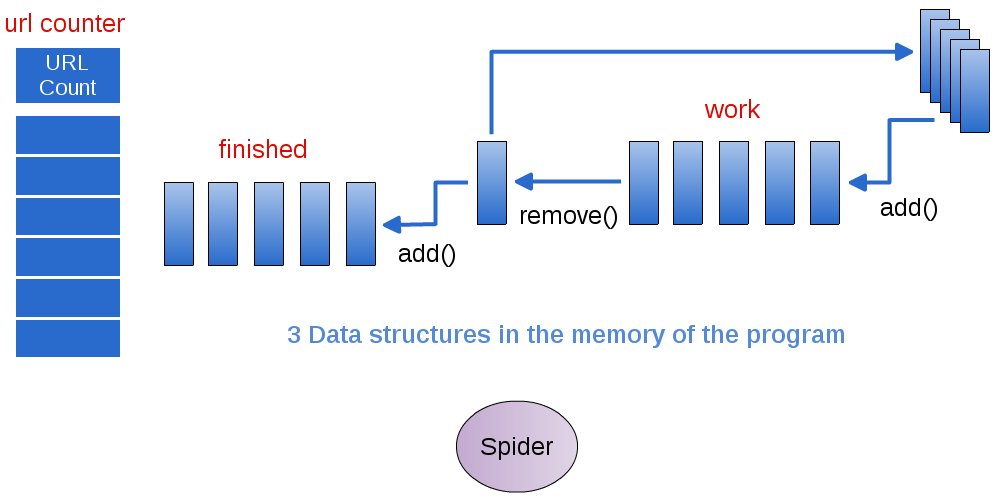
\includegraphics{Spider1.png}
\caption{Single Spider accesses the data and does all the work}\end{figure}


\section{One spider}
\label{URLSpider/URLSpider:one-spider}\begin{enumerate}
\item {} 
The original web crawling spider that you’ve been working on looks like this:

\end{enumerate}
\begin{itemize}
\item {} \begin{description}
\item[{3 data structures holding information}] \leavevmode\begin{itemize}
\item {} 
Accessed individually by the Spider class

\end{itemize}

\end{description}

\item {} 
The Spider class does all the work, one step at a time

\item {} \begin{description}
\item[{In this case, the ‘work’ is piling up!}] \leavevmode\begin{itemize}
\item {} 
Each page that is visited has many more links to follow

\end{itemize}

\end{description}

\end{itemize}
\begin{enumerate}
\setcounter{enumi}{1}
\item {} 
What might make this process faster so that more work gets done?

\end{enumerate}


\section{Executing concurrently}
\label{URLSpider/URLSpider:executing-concurrently}\begin{figure}[htbp]
\centering
\capstart

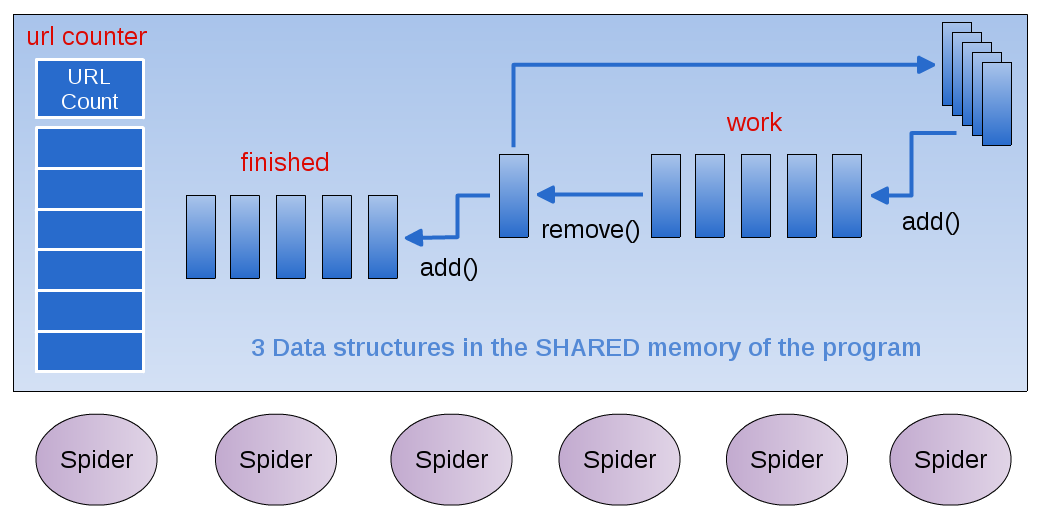
\includegraphics{Spider2.png}
\caption{Multiple Spider ‘Runnable’ Threads all access the shared data}\end{figure}


\section{Multiple Spider `threads'}
\label{URLSpider/URLSpider:multiple-spider-threads}\begin{itemize}
\item {} \begin{description}
\item[{What happens when several threads need to read and write from the ‘work’ data structure?}] \leavevmode\begin{itemize}
\item {} 
Imagine yourself as a spider working with a group of others

\item {} \begin{description}
\item[{What actions are involved when you:}] \leavevmode\begin{itemize}
\item {} 
Grab a new page to work on from the work data structure

\item {} 
Save new links to the ‘work’ data structure

\item {} 
Store the completed page in ‘done’ data structure

\end{itemize}

\end{description}

\end{itemize}

\end{description}

\end{itemize}


\section{Key point: locking}
\label{URLSpider/URLSpider:key-point-locking}\begin{itemize}
\item {} \begin{description}
\item[{For certain operations on a shared data structure,}] \leavevmode\begin{itemize}
\item {} 
Other threads must be barred from accessing when another thread is executing that operation

\end{itemize}

\end{description}

\item {} 
These operations must be atomic: only one thread can be executing this operation at a time

\item {} 
Which operations on the work data structure should be atomic?

\end{itemize}


\section{How to do this in Java}
\label{URLSpider/URLSpider:how-to-do-this-in-java}

\subsection{Creating Threads in Java}
\label{URLSpider/URLSpider:creating-threads-in-java}\begin{itemize}
\item {} 
Build a class that implements the Runnable interface:

\end{itemize}

\begin{Verbatim}[commandchars=\\\{\}]
public interface Runnable \PYGZob{}
        abstract public void run();
\PYGZcb{}
\end{Verbatim}
\begin{itemize}
\item {} 
In a class containing ‘main’, create each thread and pass it a new instance of the Runnable class

\end{itemize}


\subsection{Sharing the Data}
\label{URLSpider/URLSpider:sharing-the-data}\begin{itemize}
\item {} 
Create your shared data structures in a separate class

\item {} 
Create one instance of the shared data class in the ‘main’ class

\item {} 
Pass that instance of the shared data to each instance of the Runnable class via the constructor

\end{itemize}


\subsection{The Shared Data}
\label{URLSpider/URLSpider:the-shared-data}\begin{itemize}
\item {} 
Java has special data structures designed to be shared by Threads

\item {} 
See the documentation for \href{http://java.sun.com/j2se/1.5.0/docs/api/java/util/concurrent/package-summary.html}{java.util.concurrent}

\item {} \begin{description}
\item[{We’re using:}] \leavevmode\begin{itemize}
\item {} 
ArrayBlockingQueue

\item {} 
ConcurrentLinkedQueue

\item {} 
(ConcurrentHashMap, inside another class provided for you to hold the counts of the URLs)

\end{itemize}

\end{description}

\end{itemize}
\setbox0\vbox{
\begin{minipage}{0.95\linewidth}
\textbf{Dig Deeper:}

\medskip


Once you’ve implemented your solution,
\begin{enumerate}
\item {} 
Roughly determine the speedup of your threaded version

\end{enumerate}
\begin{itemize}
\item {} 
For varying numbers of threads

\item {} 
What will you need to measure?

\end{itemize}
\begin{enumerate}
\setcounter{enumi}{1}
\item {} 
Write a short report analyzing the speedup of your threaded solution

\end{enumerate}
\end{minipage}}
\begin{center}\setlength{\fboxsep}{5pt}\shadowbox{\box0}\end{center}


\chapter{Improving the ‘Spider’}
\label{SpiderLabpart2/SpiderLabpart2:improving-the-spider}\label{SpiderLabpart2/SpiderLabpart2::doc}

\section{First Question: How much work is there?}
\label{SpiderLabpart2/SpiderLabpart2:first-question-how-much-work-is-there}
Once you have a completed working spider, let’s examine how much
work it has to do.  Try some experiments in which you continue
using increasing values of maxUrls in the Spider.  Please note that
you can provide this value in its constructor.  Add a method to the
Spider that enables you to ask how many pages are still left to
work on in the ‘work’ queue.  You may also want to add a method to
know how many pages have been finished.

Change the RunSpider class to run some experiments with different
values of maxUrls by executing several Spiders.  For each value of
maxUrls, report on how much work is left to do.  How quickly is our
Spider overloaded with work?


\section{Multiple Spiders to the rescue}
\label{SpiderLabpart2/SpiderLabpart2:multiple-spiders-to-the-rescue}
Now let’s examine how we can use multiple spiders working at the
same time on this problem.  Your instructor will take a moment to
explain how we will use a technique called threads to run many
spiders at the same time, each of who will access the work,
finished, and urlCounter queue.  Then you will try this out below.

There is now a new lab.concurrentSpider package in our shared
space.  Examine the RunThreadedSpider class.  Note that we now use
a Java class called a Thread to begin running multiple instances of
the Spider in many Threads.  The Spider is now in a class called
ConcurrentSpider, and implements an interface called Runnable.

A key feature of concurrently running Spiders is that they must
share the same data structures in order to work together.  To do
this, we need to place the data structures they are working on in
one class and create one instance of that class in
RunConcurrentSpider.  Then each new ‘Runnable’ ConcurrentSpider
will receive a reference to that class of shared data structures.


\section{First try:  share our original data structures}
\label{SpiderLabpart2/SpiderLabpart2:first-try-share-our-original-data-structures}
We are gong to try this process in 2 steps, so you will first look
at the ‘first version’, where we will try to share the original
data structures designed for the single Spider.  Examine the
RunConcurrentSpider1 and ConcurrentSpider1 classes.  Create the
class called SharedSpiderData1 and move the data structures into it
from your original Spider class from the lab.spider package.  Make
getters for each data structure (work, finished, urlCounter).

Finish the ConcurrentSpider1 class by filling in the code needed in
run() and the processPage() method-- this should be much like you
did it for the ‘sequential’ single Spider case.  You should be able
experiment with your new ConcurrentSpider1 by running
RunThreadedSpider1.  Try running it several times without changing
anything.  Can you tell if you get the same results each time?

\begin{notice}{note}{Note:}
The following classes are needed for this first try:
\begin{itemize}
\item {} 
AllWordsCounter

\item {} 
ConcurrentSpider1

\item {} 
HTMLHelper

\item {} 
RunThreadedSpider1

\item {} 
TestHTTPHelper

\item {} 
WordsCount

\end{itemize}

You will make the SharedSpiderData1 class.
\end{notice}


\section{Second try: concurrent data structures}
\label{SpiderLabpart2/SpiderLabpart2:second-try-concurrent-data-structures}
Your instructor will discuss an important improvement in class and
share come more code with you.

Following that discussion, now use the new Java Concurrent Data
Structures from the package java.util.concurrent.  Begin with the
file SharedSpiderData to see the types of shared, thread-safe data
structures we will use for this version of the multi-threaded
crawler.

Finish the classes called ConcurrentSpider and RunThreadedSpider.



\renewcommand{\indexname}{Index}
\printindex
\end{document}
